\documentclass[a4paper,12pt]{report}
\usepackage[utf8]{inputenc}
\usepackage{graphicx}
\usepackage{geometry}
\usepackage{hyperref}
\usepackage{fancyhdr}
\usepackage{setspace}
\usepackage{tocloft}
\usepackage{xcolor}
\usepackage{tikz}
\usepackage{soul}
\usepackage{adjustbox}
\usepackage[french]{babel}
\usepackage[utf8]{inputenc}
\usepackage{caption}
\usepackage{float}



\geometry{left=2.5cm,right=2.5cm,top=2.5cm,bottom=2cm}
\setstretch{1.5}  % Line spacing

\pagestyle{plain}
\begin{document}

%----------------- Title Page -------------------
\begin{titlepage}
    \begin{center}
    
    %------------- Logo Section -------------
    \begin{minipage}[t]{0.45\textwidth}
        \raggedright
        
\includegraphics[width=8cm]{unnamed.jpg} % Replace with the path to the university logo
    \end{minipage}
    \begin{minipage}[t]{0.45\textwidth}
        \raggedleft
        
\includegraphics[width=4cm]{images.png} % Replace with the path to the enterprise logo
    \end{minipage}

    %------------- Blue Box Section -------------
    \vspace{4cm}
    \begin{tikzpicture}
    \node[draw=blue, fill=blue!40, thick, text width=0.9\textwidth, inner sep=10pt, align=center] {
        \Large
        \textbf{Rapport du stage ouvrier}\\[0.5cm]
        1\textsuperscript{ère} ACI ISITD \\[0.5cm]
        Année Universitaire : 2023/2024\\[0.5cm]
        \normalsize
        Le créneau du stage : \textbf{Thechnologies Web, Développment web, Annalyse des données }\\
      
    };
\end{tikzpicture}


    %------------- Student and Tutor Section -------------
    \vfill
    \Large\textbf{Étudiant :}\\
    \large M. : EZZARI Abdellah (Groupe B)\\[1cm]

    \Large\textbf{Nom du tuteur :}\\
    \large Mme.HADDOUZ Kawtar
    
    \end{center}
\end{titlepage}


%----------------- Remerciements -------------------
\chapter*{Remerciements}
\addcontentsline{toc}{chapter}{Remerciements}
% Write your acknowledgements here
 Je tiens à vous exprimer mes sincères remerciements pour l’accueil chaleureux et l’encadrement bienveillant que vous m’avez accordé durant mon stage au sein d’OCP Group à Youssoufia. Mme.Haddouz Kawtar, en tant que ma tutrice, votre disponibilité et vos conseils précieux ont été d’une grande aide pour mieux comprendre les aspects pratiques de ce métier. Mr.El Faiq Mustapha, votre rôle en tant qu’encadrant a été déterminant pour approfondir mes connaissances techniques et me guider à travers les diverses missions confiées. Grâce à vos accompagnements respectifs, cette expérience a été à la fois formatrice et enrichissante, et je vous en suis profondément reconnaissant(e).

Je voudrais également exprimer ma profonde reconnaissance envers ma famille, dont le soutien infaillible m’a été d’une grande aide tout au long de cette expérience.

Enfin, je tiens à remercier chaleureusement l’École des Sciences de l’Information, ses professeurs et cadres académiques, pour leur accompagnement et leur rôle essentiel dans ma formation. Leur enseignement et leurs encouragements m’ont préparé à tirer le meilleur parti de cette opportunité de stage.

Je garderai un excellent souvenir de cette période passée au sein d'OCP Group, et je vous remercie vivement pour la confiance que vous m’avez accordée.

%----------------- Résumé -------------------
\chapter*{Résumé}
\addcontentsline{toc}{chapter}{Résumé}

% Write your summary here
Lors de mon stage, j'ai eu l'opportunité de travailler sur un projet à la fois important et enrichissant. Ma mission principale consistait en \textbf{le développement d'une application web dédiée à la gestion des équipements individuels de sécurité}. Ce projet m'a permis de m'impliquer dans plusieurs tâches essentielles qui ont contribué à son succès.

Tout d'abord, j'ai été chargé de \textbf{l'analyse des besoins} afin de sélectionner la technologie la plus adaptée au projet. Cette étape a nécessité une compréhension approfondie des exigences fonctionnelles et techniques. Cela m'a permis de renforcer mes compétences en analyse et en prise de décision.

Ensuite, j'ai participé à \textbf{la création de la base de données} en exploitant des fichiers Excel existants. Cette tâche incluait la préparation et l'analyse des données pour assurer leur intégrité et leur pertinence.

De plus, j'ai été impliqué dans des \textbf{sorties vers d'autres entités de travail}, ce qui m'a permis de comprendre les interactions entre différents départements et de m'adapter à divers environnements professionnels. Cette expérience a renforcé ma capacité à collaborer efficacement avec des équipes multidisciplinaires.

Enfin, j'ai eu l'occasion d'\textbf{assister à des réunions}, ce qui m'a offert un aperçu précieux des processus décisionnels et des stratégies de gestion de projet. Cela m'a également aidé à développer mes compétences en communication et en présentation.

Ce stage a été une opportunité précieuses pour mettre en pratique les compétences et connaissances acquises tout au long de l'année universitaire. Il m'a permis d'appliquer mes acquis théoriques dans un contexte professionnel réel et de développer de nouvelles compétences techniques et organisationnelles. Grâce à cette expérience, j'ai gagné en confiance et en autonomie, ce qui me prépare davantage pour mes futures responsabilités professionnelles.

\newpage


%----------------- Table of Contents -------------------
\tableofcontents
\newpage


%----------------- Liste des figures -------------------

\addcontentsline{toc}{chapter}{Liste des figures}
\listoffigures



\newpage

%----------------- List of Abbreviations -------------------
\chapter*{Liste des Abréviations}
\addcontentsline{toc}{chapter}{Liste des Abréviations}
     — \textbf{HSE}: Hygiène, Sécurité et Environnement.
     
     — \textbf{OCP}: Office Chérifien des Phosphates.
     
     — \textbf{HSES}: Hygiène, Sécurité, Environnement et Site.
     
     — \textbf{HSEE}: Hygiène, Sécurité, Environnement et Entité.
     
     — \textbf{PHP}: Hypertext Preprocessor.
% Add a list of abbreviations here, if necessary

%----------------- Introduction -------------------
\chapter*{Introduction}
\addcontentsline{toc}{chapter}{Introduction}
% Write your introduction here
\section{Contexte du satge :}
Ce stage d’initiation a été réalisé au sein de l’entreprise OCP Group, à Youssoufia, plus précisément dans l’entité Laverie(responsable du processus de lavage du phosphate) chez le service HSE (Hygiène, Sécurité et Environnement). OCP Group, acteur majeur de l'industrie des phosphates et dérivés, offre un cadre stimulant pour l'apprentissage et l'intégration des normes de sécurité et de gestion environnementale dans un environnement industriel. Mon stage, qui s'est déroulé du 1er juillet 2024 au 29 juillet 2024.
\section{Objectifs :}
 Les principaux objectifs de ce stage étaient les suivants :
 
 — Découvrir le monde professionnel et s’intégrer dans un environnement de travail
 dynamique.
 
 — Comprendre le fonctionnement et les besoins spécifiques du Group OCP Youssoufia.
 
 — Acquérir des compétences techniques en développement d’applications avec PhP et son framework Laravel .
 
 — Réaliser une application pour la gestion des EPI et des dotations générale et  exceptionnelles .

 — Mettre en œuvre la fonctionnalité de generations des dotations en se basant sur les 
 données entrées par l'employeur du service HSE.
\section{Présentation de l'organisme d'accueil :}
\subsection{OCP GROUP :}
L’OCP est une société anonyme dénommée “OCP S.A” depuis 2008, fondé en 1920, et dirigé par monsieur Mostafa TERRAB, occupe une place particulière dans l’histoire industrielle du Maroc. Le Groupe est le premier exportateur de minerai au monde, leader sur le marché de l’acide phosphorique et acteur majeur dans les engrais solides.
Désormais ayant plus de 150 clients dans le monde et doté d’une culture
entrepreneuriale forte et d’une stratégie industrielle incontournable, l’OCP dispose d’une occasion certaine pour poursuivre son développement de manière durable : le chiffre d’affaires du groupe en 2023 s’élève à 91,27 milliards de DH et emploie plus de 23 000 collaborateurs.
\subsection{Histoire :}
La première découverte de phosphate au Maroc remonte à 1905. C’était dans le bassin des Meskala, au centre du pays. Elle n’avait alors pas suscité un intérêt notable. La découverte de phosphate exploitable a eu lieu en 1917 à Oued Zem, dans le nord du pays, lors de travaux de terrassement d’une voie de chemin de fer.
Depuis cette date l’office n’a cessé de renforcer la place qu’il occupe dans l’industrie des phosphates et de ses dérivées, c’est ainsi qu’indépendamment de sa place traditionnelle de premier exportateur de phosphate naturel, le groupe O.C.P. a accédé en 1982 au rang de premier exportateur mondial d’acide phosphorique concentré en 54 % P2O5.
Ainsi dès sa création, le 7 août 1920, l’O.C.P. a été constitué sous la forme d’un organisme d’état à caractère industriel et commercial doté d’une organisation du type société privée. L’évolution de ses activités et l’ampleur de ses projets de vaporisation ont conduit à la mise en Place en 1975, d’une structure de Groupe permettant l’intégration de différentes entités complémentaires au sein d’un même ensemble.

1920 : Création de l'OFFICE CHERIFIEN DES PHOSPHATES (OCP) le 7août 1920.

1931 : Début de l’extraction en souterrain à Youssoufia.

1936 : Premier train de phosphate de Youssoufia vers le port de Safi.

1942 : Création d'une unité de calcination à Youssoufia.

1954 : Démarrage des premières installations de séchage à YOUSSOUFIA. 

1962 : Introduction de la mécanisation du souterrain à Youssoufia.

1969 : Entrée en exploitation de la première Recette de phosphate noir à Youssoufia.

1975 : Création du Groupe OCP.

2005 : création de la laverie.
\begin{figure}[h]
    \centering
    \fbox{\adjustbox{valign=t, margin=1em 2em}{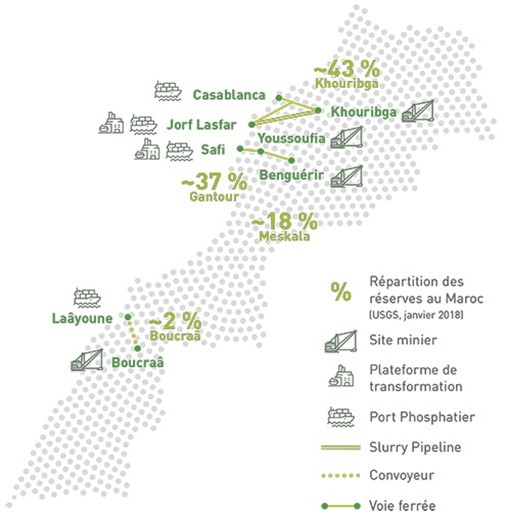
\includegraphics[width=0.6\textwidth]{Picture4.jpg}}}
    \caption{Localisation de OCP au Maroc .}
    \label{fig:mon_image}
\end{figure}
\subsection{L'activité et le rôle économique de Group OCP :}
L'activité du groupe OCP repose sur 8 étapes principales. Ces opérations couvrent l'ensemble de la chaîne de valeur des phosphates, depuis l'extraction minière jusqu'à l'exportation, en passant par la transformation industrielle. Le groupe opère sur quatre sites miniers, deux sites de transformation, et un réseau d'installations portuaires. OCP continue d'améliorer l'efficacité des processus tout en réduisant les coûts énergétiques et en ressources, permettant ainsi de maximiser la valeur des phosphates.

Dans le cadre de sa démarche vers un avenir durable, le groupe OCP a développé des solutions innovantes pour l'extraction et le transport des phosphates, réduisant ainsi considérablement la consommation d'eau, d'énergie et de phosphate. Grâce à ces améliorations technologiques et de processus, le groupe réussit à produire plus avec moins.

Le Maroc a enregistré des progrès considérables dans l'industrie des phosphates depuis son indépendance en 1956. Ces progrès concernent notamment :

\begin{itemize}
  \item L'étude des gisements et des minerais,
  \item La mécanisation de l'extraction à ciel ouvert et souterrain,
  \item La diversification des méthodes de traitement du minerai,
  \item La chimie des phosphates,
  \item La formation du personnel.
\end{itemize}


\begin{figure}[h]
    \centering
    \fbox{\adjustbox{valign=t, margin=1em 2em}{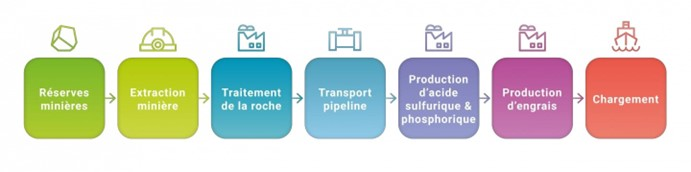
\includegraphics[width=0.6\textwidth]{Picture2.jpg}}}
    \caption{Localisation de OCP au Maroc .}
    \label{fig:mon_image}
\end{figure}

L'OCP joue un rôle crucial sur le plan socio-économique, employant plus de 24.000 agents répartis dans ses différents centres au Maroc. Au sein de la Direction de l'Industrie et des Jardins (DIJ), l'effectif total est d'environ 3.200 agents.

\textbf{Répartition des effectifs par catégorie :}

Cet établissement semi-public à caractère industriel et commercial occupe une position importante tant à l'échelle nationale qu'internationale. En 2018, sa capacité de production a atteint 270 millions de tonnes de phosphates par an, représentant plus de 90 pour cent  des revenus de l'industrie minière marocaine. L'OCP est également reconnu comme le premier exportateur mondial de phosphates, avec une part de marché de 28 pour cent sous toutes ses formes.
\begin{figure}[h]
    \centering
    \fbox{\adjustbox{valign=t, margin=1em 1em}{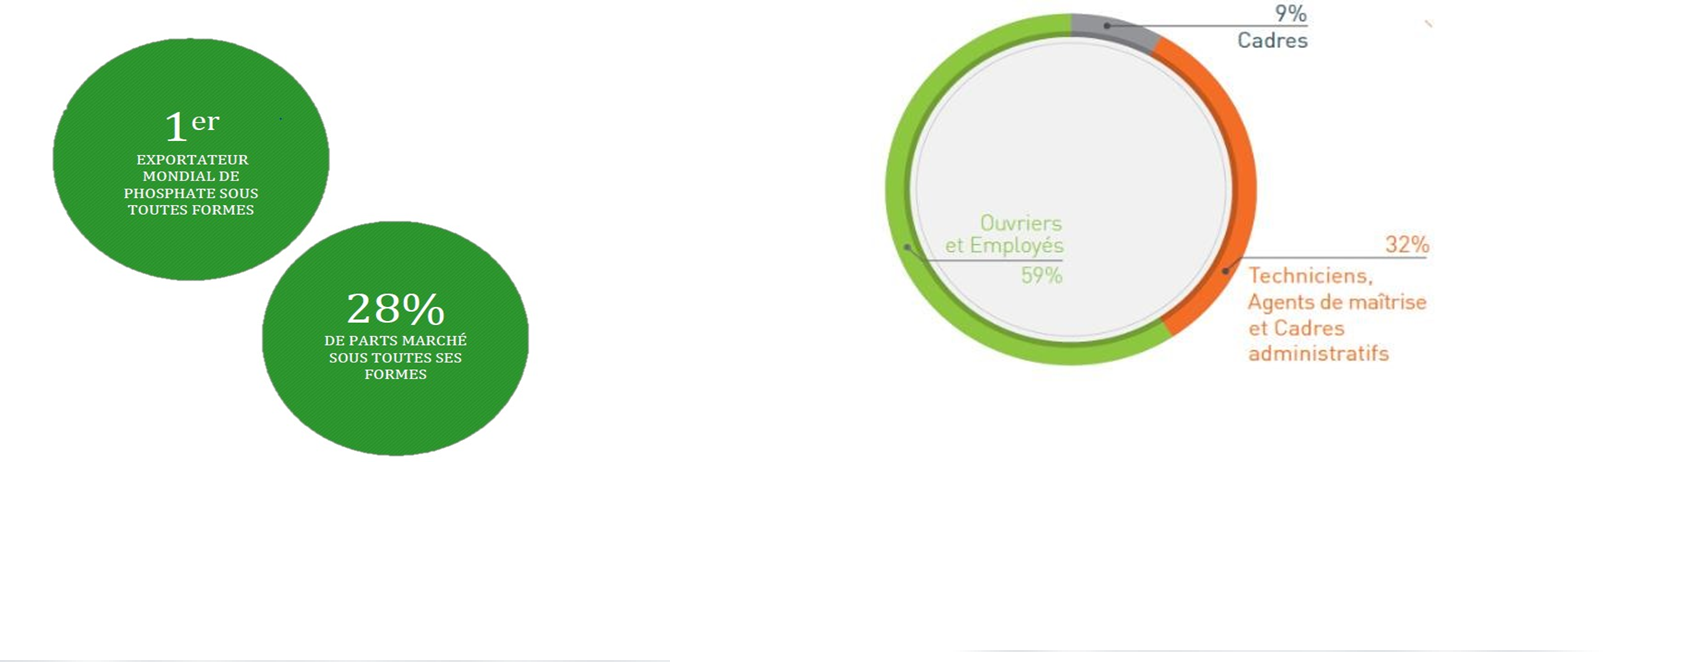
\includegraphics[width=0.6\textwidth]{Picture5.png}}}
    \caption{Rôle économique de OCP Group .}
    \label{fig:mon_image}
\end{figure}


\newpage



\subsection{Organigrammes :}
\begin{figure}[h]
    \centering
    \fbox{\adjustbox{valign=t, margin=1em 2em}{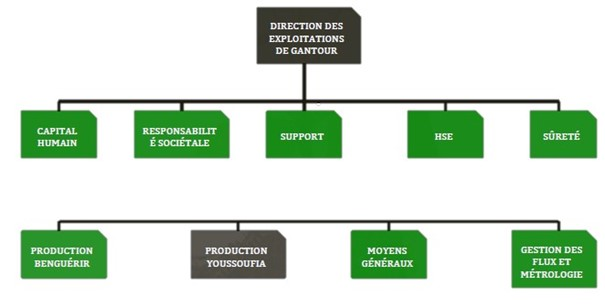
\includegraphics[width=0.6\textwidth]{Picture3.jpg}}}
    \caption{l'organigramme de l'organisation OCP .}
    \label{fig:mon_image}
\end{figure}

\begin{figure}[h]
    \centering
    \fbox{\adjustbox{valign=t, margin=1em 2em}{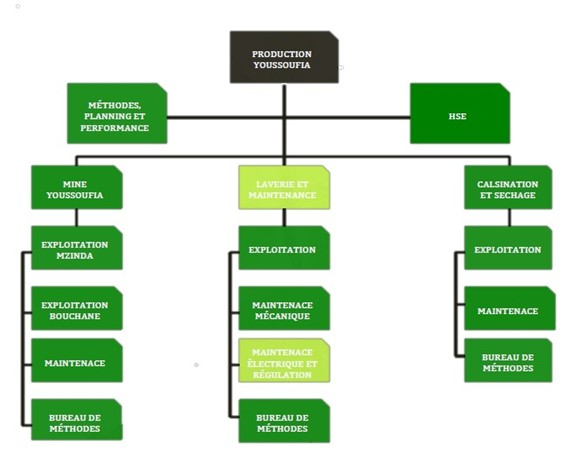
\includegraphics[width=0.6\textwidth]{Picture1.jpg}}}
    \caption{organigrammes de site de production Youssoufia .}
    \label{fig:mon_image}
\end{figure}
\newpage
\subsection{Presentation de l'entité laverie :}
L'entité Laverie de l'OCP Group à Youssoufia est un site industriel spécialisé dans le traitement du phosphate brut. Son rôle est d'éliminer les impuretés comme l'argile et le sable à travers un processus de lavage, ce qui permet d'améliorer la qualité du phosphate pour sa production d’engrais ou son exportation.

Le site utilise des équipements industriels sophistiqués et de grandes quantités d'eau, nécessitant une gestion rigoureuse des ressources et des infrastructures. La Laverie joue un rôle crucial dans la chaîne de valeur du phosphate, contribuant de manière significative à l'économie locale et à l'industrie mondiale des phosphates.

Au sein du service HSE (Hygiène, Sécurité, Environnement) de la Laverie, le HSES site supervise toutes les autres équipes HSE, appelées HSEE entité. En tant que stagiaire en informatique, j'ai été impliqué dans la gestion des systèmes liés à l'entrée et à la sortie des équipements individuels de sécurité, contribuant ainsi à l'amélioration de la gestion des équipements de protection au sein du site.
\begin{figure}[h]
    \centering
    \fbox{\adjustbox{valign=t, margin=1em 2em}{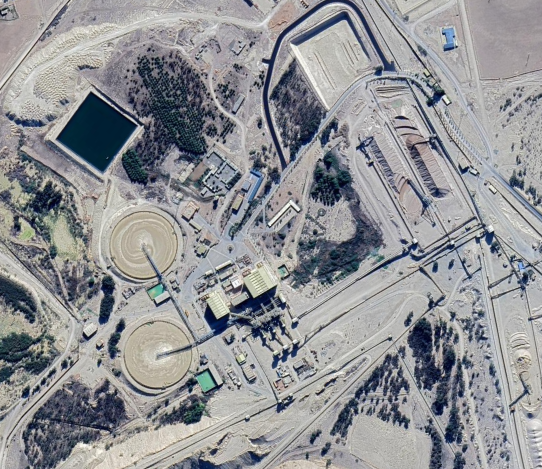
\includegraphics[width=0.6\textwidth]{Screenshot 2024-09-16 155025.png}}}
    \caption{Entité Laverie .}
    \label{fig:mon_image}
\end{figure}





%----------------- Développement -------------------
\chapter*{L'application "EPI.ation" :}
\addcontentsline{toc}{chapter}{Web application "EPI.ation"}
\section{Présentation de l'application}

\textbf{"EPI.ation"} est une application web déployée localement. Cette application a été développée pour répondre aux besoins de la transformation digitale au sein du service HSE de l'entreprise où j'ai effectué mon stage. La problématique était la nécessité de digitaliser le processus de génération des dotations après la distribution des équipements de sécurité.

\subsection{Technologies Utilisées}

Le choix des technologies est crucial pour le succès de tout projet de développement logiciel. Voici les principaux outils et frameworks que j'ai utilisé :

\subsubsection{PHP}

PHP est un langage de script côté serveur que nous avons choisi pour développer l'application "EPI.ation" en raison de sa capacité à créer des applications web dynamiques et interactives. Sa simplicité et sa flexibilité sont idéales pour un développement rapide, que ce soit pour des prototypes ou des applications à grande échelle. Étant largement supporté et bénéficiant d'une vaste communauté, PHP facilite la résolution de problèmes et l'accès à des ressources variées, ce qui est crucial pour assurer la robustesse et l'évolution de notre application dans le cadre de la transformation digitale du service HSE.

\subsubsection{Laravel}
\begin{figure}[H]
    \centering
    \fbox{
\includegraphics[width=0.5\textwidth]{framework-php-laravel-logo.png}}
    \caption{Logo de l'application}
\end{figure}

Laravel, un framework PHP moderne, a été utilisé pour simplifier le développement de notre application web grâce à son architecture MVC (Modèle-Vue-Contrôleur). Cette structure organisée permet de maintenir un code propre et modulaire, facilitant ainsi la gestion des évolutions et des modifications. Laravel offre des fonctionnalités telles que l'Eloquent ORM pour la gestion des bases de données, un système de routage intuitif, et des outils de migration. Ces éléments ont été essentiels pour gérer les données de dotation et garantir la sécurité avec des mécanismes intégrés comme la protection CSRF et l’authentification, répondant ainsi aux besoins spécifiques du service HSE.

\subsubsection{MySQL}
\begin{figure}[H]
    \centering
    \fbox{
\includegraphics[width=0.5\textwidth]{download.jpg}}
    \caption{Logo de l'application}
\end{figure}

Pour la gestion des données, nous avons opté pour MySQL, un système de gestion de bases de données relationnelles (SGBDR) très populaire. MySQL est reconnu pour sa fiabilité, sa performance, et sa facilité d'utilisation. Il permet de gérer efficacement les informations relatives aux employés et aux équipements de sécurité tout en assurant leur intégrité et leur sécurité. Son intégration facile avec PHP et Laravel a fait de MySQL un choix naturel pour notre projet, permettant un suivi précis des dotations et des allocations au sein du service HSE.

\subsubsection{Bootstrap}
\begin{figure}[H]
    \centering
    \fbox{
\includegraphics[width=0.5\textwidth]{1605445072.png}}
    \caption{Logo de l'application}
\end{figure}

Bootstrap a été utilisé pour concevoir une interface utilisateur réactive et esthétique. Ce framework CSS offre une vaste collection de composants prêts à l'emploi, tels que des boutons, des formulaires, et des barres de navigation, ce qui a accéléré le processus de développement. De plus, Bootstrap assure la compatibilité de l'application avec différents appareils et tailles d'écran, améliorant ainsi l'expérience utilisateur et facilitant l'accès aux fonctionnalités par le personnel du service HSE.

\subsubsection{Dompdf}

Pour les fonctionnalités de génération de documents, nous avons intégré Dompdf, un package PHP permettant de convertir le HTML et le CSS en fichiers PDF. Cette bibliothèque est particulièrement utile pour créer des rapports et des factures dynamiques que les utilisateurs peuvent télécharger directement depuis l'application. Dompdf simplifie la création de PDF en permettant l’utilisation de styles CSS pour la mise en page, assurant ainsi une cohérence visuelle avec le reste de l’application et répondant aux besoins administratifs du service HSE.

\vspace{1cm}
\begin{figure}[H]
    \centering
    \fbox{
\includegraphics[width=0.5\textwidth]{F.png}}
    \caption{Logo de l'application}
\end{figure}

\subsection{Diagrammes UML}

\subsubsection{Diagramme de Cas d'Utilisation}

Le diagramme de cas d'utilisation pour le service HSE illustre les principales interactions entre les utilisateurs (tels que les agents de sécurité et les gestionnaires de l'équipement) et le système. Les cas d'utilisation incluent la connexion au système, la saisie des informations sur l'équipement de sécurité, et la génération des dotations pour assurer une distribution adéquate des équipements de protection individuelle (EPI). Ce diagramme aide à identifier les fonctionnalités essentielles que l'application doit offrir pour soutenir les opérations HSE, en garantissant que tous les utilisateurs peuvent accéder aux outils nécessaires pour maintenir des normes de sécurité élevées.

\vspace{1cm}
\begin{figure}[H]
    \centering
    \fbox{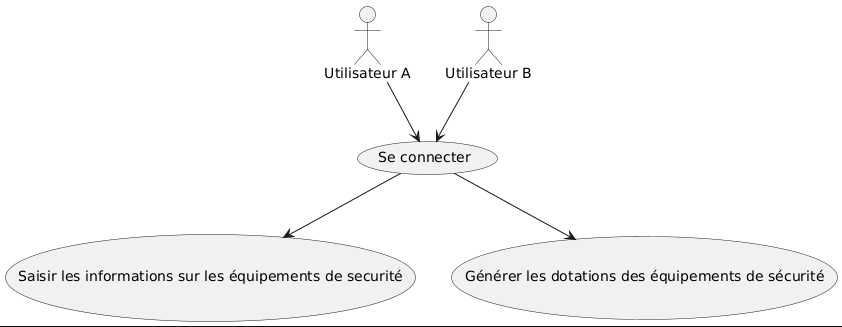
\includegraphics[width=0.8\textwidth]{Screenshot 2024-09-18 204545.png}}
    \caption{Diagramme de Cas d'Utilisation}
\end{figure}

\subsubsection{Diagramme de Classes}

Le diagramme de classes fournit une vue détaillée de la structure de l'application HSE, montrant comment les données sont organisées et interconnectées. Les principales classes incluent Utilisateur, qui représente les différents acteurs utilisant le système, Équipement, qui stocke les détails des EPI, et Dotation, qui gère l'allocation de ces équipements aux utilisateurs. Ce diagramme est crucial pour les développeurs, car il définit la structure des données et les relations entre les différentes entités, assurant ainsi que l'application puisse gérer efficacement les informations critiques pour le service HSE.

\vspace{1cm}
\begin{figure}[H]
    \centering
    \fbox{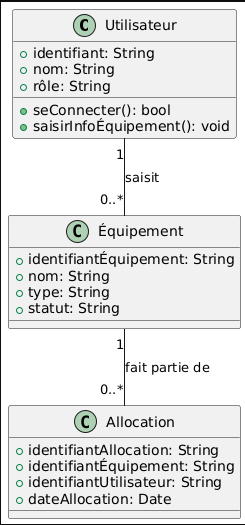
\includegraphics[width=0.4\textwidth]{123.png}}
    \caption{Diagramme de Classes}
\end{figure}

\subsubsection{Diagramme de Séquence}


\vspace{1cm}
\begin{figure}[H]
    \centering
    \fbox{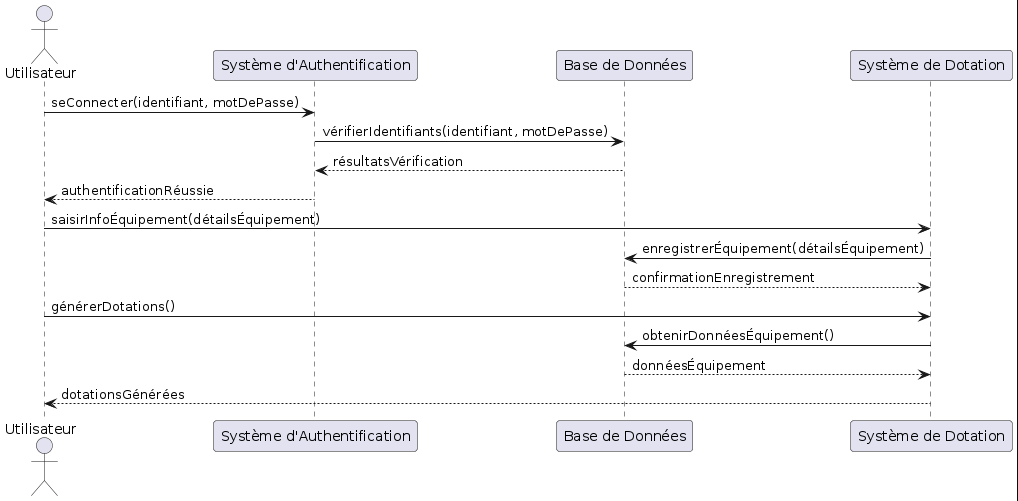
\includegraphics[width=1\textwidth]{1123.png}}
    \caption{Diagramme de Séquence}
\end{figure}

Le diagramme de séquence décrit le flux d'interactions dynamiques entre les composants du système lors de l'exécution des tâches clés, telles que la connexion, la saisie des informations sur l'équipement, et la génération des dotations. Il montre comment les utilisateurs interagissent avec le système d'authentification, le système de dotation, et la base de données. Ce diagramme est essentiel pour comprendre l'ordre des opérations et les échanges de messages nécessaires pour accomplir les processus métier du service HSE, garantissant ainsi une gestion fluide et efficace des équipements de sécurité et de la conformité réglementaire.

\chapter*{Conclusion}
\addcontentsline{toc}{chapter}{Conclusion}


Mon stage au sein du service HSE de l'OCP Group Youssoufia m’a permis de mettre en pratique les compétences acquises durant ma formation académique, tout en me confrontant aux réalités d’un environnement professionnel. Le projet de digitalisation du processus de gestion des dotations d’équipements de sécurité, à travers le développement de l’application "EPI.ation", a été une expérience enrichissante tant sur le plan technique que personnel. J’ai pu renforcer mes compétences en développement web avec PHP et Laravel, tout en intégrant des technologies modernes comme Bootstrap et Dompdf pour répondre aux besoins spécifiques du service.

Ce projet m'a non seulement permis de contribuer à la transformation digitale du service HSE, mais il m'a également aidé à mieux comprendre l’importance d’un processus structuré et sécurisé dans la gestion des équipements de sécurité. Grâce à l’accompagnement de mes encadrants et aux échanges avec les équipes sur le terrain, j’ai pu évoluer dans un cadre collaboratif et stimulant.

Je ressors de cette expérience avec une meilleure maîtrise des outils technologiques et des méthodologies de gestion de projet, ainsi qu'une compréhension accrue des enjeux liés à la sécurité au travail. Ce stage a renforcé ma volonté de continuer à développer mes compétences dans le domaine des technologies de l’information, en particulier dans des environnements industriels.

%----------------- Annexes -------------------
\appendix
\chapter*{Annexes}
\addcontentsline{toc}{chapter}{Annexes}

       \textbf{Tous les codes du projet réalisés au cours du stage :}
       
        \begin{itemize}
        \item \href{https://github.com/ABDOx500/EPI_Intership_1ACI.git}{Projet réalisé au cours du stage}
        \end{itemize}
         \textbf{le codes Latex utiliser pour création du rapport de mon stage :}
         
        \begin{itemize}
        \item \href{https://github.com/ABDOx500/stage_1_ACI.git}{Projet réalisé au cours du stage}
        \end{itemize}

\end{document}
